\documentclass[letterpaper,twocolumn,10pt]{article}
\usepackage{usenix-2020-09}
\usepackage{xcolor}
\usepackage[inline]{enumitem}
\usepackage{stfloats}
\usepackage{makecell}

\usepackage{hyperref}      % (don’t load twice)
\usepackage{xurl}          % allow breaks at many characters

\usepackage[dvipsnames]{xcolor}
\definecolor{DarkLink}{HTML}{0A58CA}

% hyperref is already loaded by the class
\hypersetup{
  colorlinks=true,
  linkcolor=DarkLink,
  citecolor=DarkLink,
  urlcolor=DarkLink,
  breaklinks=true
}

\usepackage{amsmath}
\usepackage{listings}
\usepackage{bm}
\usepackage{xcolor}
\usepackage{color}
\usepackage{xspace}
\usepackage{graphicx}
\usepackage{subcaption}
\usepackage{svg}
\usepackage{booktabs}
\usepackage[ruled,vlined,linesnumbered]{algorithm2e}
\usepackage{enumitem}
\usepackage{todonotes}


\usepackage[normalem]{ulem}
% \usepackage[normalem]{ulem} % strikethrough
% \usepackage{sidecap}
\usepackage{multirow}
\usepackage[font=small,labelfont=bf]{caption}

\usepackage{siunitx}        % new, for nicer aligning of numbers in table
\usepackage{etoolbox}       % new, for making command \bfseries robust
\usepackage{booktabs}
\usepackage{cleveref}
\usepackage{bbm}         % for mathbbm


\renewcommand{\sectionautorefname}{Section}
\renewcommand{\subsectionautorefname}{Subsection}
\renewcommand{\subsubsectionautorefname}{Subsection}
\renewcommand{\chapterautorefname}{Chapter}
\renewcommand{\figureautorefname}{Figure}
\renewcommand{\tableautorefname}{Table}
\renewcommand{\equationautorefname}{Equation}
\renewcommand{\algorithmautorefname}{Algorithm}


% % Spacing
\usepackage{titlesec}
\titlespacing\section{0pt}{6pt}{2pt}
\titlespacing\subsection{0pt}{4pt}{2pt}
\titlespacing\subsubsection{0pt}{4pt}{2pt}
\titlespacing\paragraph{0pt}{4pt}{4pt}

% Make all lists tighter
\setlist{nosep}                    % = noitemsep + topsep=0pt
\setlist[itemize]{leftmargin=*}    % no extra left indent (align with text)
% \setlist{topsep=0pt, leftmargin=*}
% Optional fine-tuning:
% \setlist{itemsep=0.2ex, topsep=0.5ex, parsep=0pt, partopsep=0pt}

\def\Snospace~{\S{}}
\renewcommand*\sectionautorefname{\Snospace}
% \renewcommand\figurename{Fig.}
\renewcommand*\figureautorefname{Figure}
\renewcommand*\subsectionautorefname{\Snospace}
\renewcommand*\subsubsectionautorefname{\Snospace}
% \newcommand{\ie}{\emph{i.e.},\xspace}
% \newcommand{\eg}{\emph{e.g.},\xspace}
\DeclareMathOperator*{\argmax}{arg\,max}

\definecolor{darkgreen}{rgb}{0.0, 0.5, 0.0}

\newcommand{\sysname}{\textit{Adaptive-Marginal-Hits}\xspace}
\newcommand{\deploymentname}{\textit{CompanyX}\xspace}
\newcommand{\ta}{\textsc{Tail-Age\xspace}}
\newcommand{\erate}{\textsc{Eviction-Rate\xspace}}
\newcommand{\hps}{\textsc{Hits-Per-Slab\xspace}}
\newcommand{\mh}{\textsc{Marginal-Hits\xspace}}


\newcommand{\jason}[1]{{\color{orange}{jason: #1}}}
\newcommand{\jadd}[1]{\color{orange}{#1}}
\newcommand{\jrem}[1]{\sout{#1}}
\newcommand{\yazhuo}[1]{{\color{magenta}{yazhuo: #1}}}
\newcommand{\hongshu}[1]{{\color{teal}{hongshu:#1}}}
\newcommand{\yunjia}[1]{{\color{darkgreen}{yunjia:#1}}}
\newcommand{\fixme}[1]{{\color{red}{FIXME:#1}}}
\newcommand{\ana}[1]{{\color{blue}{ana: #1}}}
\newcommand{\pranav}[1]{{\color{purple}{pranav: #1}}}
\newcommand{\william}[1]{{\color{teal}{william: #1}}}

\newcommand{\mypar}[1]{\textbf{{#1}}}

% \renewcommand{\jason}[1]{}
% \renewcommand{\jadd}[1]{}
% \renewcommand{\jrem}[1]{}
% \renewcommand{\yunjia}[1]{}
% \renewcommand{\fixme}[1]{}

\pagestyle{plain}

\begin{document}
\date{}

% \title{Everything You Want to Know about Slab Rebalance in Memory Caches}
% \title{Slab Rebalancing in Memory Caches: Algorithms, Trade-offs, and Empirical Insights}
% \title{On the Effectiveness of Slab Rebalancing in Memory Caches}
% \title{State of Slab Rebalancing: What Works and What Doesn’t}
\title{Versioning Practice in Vector Databases}

\maketitle

\begin{abstract}
Vector databases increasingly host multiple collections whose
contents heavily overlap, such as successive corpus versions or
per-tenant overlays on a shared substrate, which raises the
question of whether the storage layer can serve them from common
data. We study this question on Milvus through two complementary
layouts. The fully replicated layout gives each tenant its own
collection and exposes the segment boundaries that stock Milvus
produces for near-identical inputs. The shared partition layout
folds the shared corpus and the tenant-private vectors into a
single collection and exposes the query throughput that arises
when tenants contend for the same physical resources. Two
benchmarks built on CodeSearchNet and Wikipedia drive the two
layouts under several Milvus configurations. The fully replicated
layout fails to share segments under stock settings because flush
jitter and size-based compaction send near-identical inputs along
divergent merge paths. The shared partition
layout, in turn, trades its storage savings for a sharp throughput
cliff under concurrent tenants, with stable refault counts and
rising per-query read volume identifying page-cache thrashing.
\end{abstract}

\section{Introduction}

Vector databases~\cite{wang2021milvus, pan2024survey} have moved
from single-tenant prototypes to shared infrastructure that serves
many collections out of the same deployment. A common pattern is
that several collections in the same cluster hold near-duplicate
data: successive versions of a corpus held side by side during a
staged rollout, filtered subsets carved out for specific tenants, or
per-tenant overlays that customize a small fraction of records on
top of a shared substrate. Because these versions overlap heavily
at the raw vector level, a multi-tenant storage layer has an
obvious opportunity to share segments and index structures across
collections rather than duplicating them end to end. Whether that
opportunity is reachable depends on two properties of today's
systems: how much segment-level redundancy actually survives the
ingest path when two near-identical collections are loaded back to
back, and how query throughput behaves once tenants are forced to
share the same physical resources for that redundant data.

This report quantifies both properties on
Milvus~\cite{wang2021milvus}. We frame two layout options for
representing a shared corpus together with per-tenant private
vectors. \emph{Fully replicated} gives each tenant its own collection
and isolates them at every layer of the storage stack at the cost
of duplicating the shared corpus across tenants. \emph{Shared
partition} keeps a single collection in which the shared corpus
and each tenant's private vectors live in distinct partitions, paying
for the shared corpus only once but forcing tenants to contend for
the same memory and page cache at query time. The fully replicated
layout raises the question of whether stock Milvus produces
segment boundaries stable enough for two near-identical collections
to be served from common segments at all. The shared partition
layout raises the question of whether the resulting resource
sharing still delivers competitive query throughput once tenants
run concurrently.

A practical obstacle to studying these questions is that existing
vector search benchmarks target single-tenant accuracy and latency
and do not expose the multi-tenant patterns described above. We
therefore construct two benchmarks on top of established corpora
to probe the two layouts. The first repurposes
CodeSearchNet~\cite{husain2019codesearchnet} from the VIBE
benchmark~\cite{vibe2024} into two near-identical collections that
differ only by a small prefix trim and is loaded under several
Milvus configurations that progressively disable jitter and
compaction, which lets us examine how the storage layer responds
to two tenants whose data is almost identical. The second carves a
Wikipedia corpus into a shared partition and two tenant partitions
under three workload variants that vary how much of the cold
vectors and queries fall on the shared partition, which lets us
examine how query behavior responds when tenants compete for the
same memory and page cache.

The measurements show that segment-level overlap under stock
Milvus is dense and scattered because flush jitter and size-based
compaction push near-identical inputs along divergent merge paths,
and that the underlying workload itself, in which top-100 ground
truth neighbors are spread across many segments per query, leaves
clear room for segment-granularity sharing once that
non-determinism is removed. The shared partition layout, in turn,
trades its storage savings for a sharp throughput cliff under
concurrent tenants, with the signature of page-cache thrashing
rather than CPU saturation. Together these results indicate that
there is real opportunity to optimize the storage layout for
multi-tenant vector databases, and that any such design must
explicitly manage the working set in the page cache rather than
rely on the current segment-per-partition layout and the operating
system's default memory management.

\section{Background}
\label{sec:background}

\subsection{Vector databases and k-nearest neighbor search}

A vector database stores high dimensional vectors that represent
unstructured records such as text passages, code snippets, or images
embedded by a learned model. The dominant query primitive is
$k$-nearest neighbor search: given a query vector, the system returns
the $k$ corpus vectors closest to it under a fixed distance metric, for
example cosine similarity or Euclidean distance. Because exhaustively
scanning every vector is prohibitive at corpus sizes of tens or
hundreds of millions, modern systems rely on approximate nearest
neighbor indices that trade a small recall loss for one or two orders
of magnitude in latency.

The literature has produced several families of approximate nearest
neighbor index, each making a different trade-off between build
time, memory footprint, query latency, and recall.
\emph{Hashing based} indices, exemplified by locality sensitive
hashing, bucket vectors so that similar points collide with high
probability, trading recall for very fast lookups.
\emph{Inverted file} indices cluster the corpus into Voronoi cells
and probe only the cells closest to the query at search time, and
are often combined with product quantization to compress each
vector down to a few bytes and shrink the resident memory footprint
at the cost of some recall. \emph{Graph based} indices, of which
HNSW~\cite{malkov2018hnsw} is the most widely deployed example,
treat each vector as a node linked to its approximate neighbors and
answer queries by greedy walks on the graph. Graph indices
currently dominate published benchmarks for in-memory approximate
nearest neighbor search. Across all of these families the
index ultimately determines which vectors a query inspects, and
therefore determines the query performance.

\subsection{LSM based search architecture}

Vector databases that ingest data continuously cannot rebuild a single
monolithic index on every write. Systems such as
Milvus~\cite{wang2021milvus} and Manu~\cite{guo2022manu} therefore
adopt a log structured merge (LSM) style layout. Incoming vectors are
first buffered in a mutable \emph{growing segment} held in memory.
When the growing segment reaches a target size it is flushed to object
storage as an immutable \emph{sealed segment}, after which a per
segment vector index, typically an HNSW graph, is built over the
flushed vectors. A collection therefore exists on disk as a sequence of
sealed segments, each carrying its own data file and its own index
structure, plus at most one growing segment in memory.

The query path mirrors this layout. A search request is fanned out to
every segment in the collection, including the growing one. Each
segment independently searches its local index and returns its own
top $k$ candidates, and a coordinator merges the per segment results
into the global top $k$ that is returned to the client. Because every
segment is consulted on every query, the per query cost scales with
the number of segments and with the size of each segment's index,
which means the segment layout, how many segments exist, how large
they are, and which vectors they contain, directly determines query
latency and the working set held in memory or page cache.
%Two further mechanisms reshape this layout in practice. First, Milvus jitters the
% flush threshold so that successive sealed segments do not all reach
% the seal point at exactly the same vector count, which prevents
% synchronized flushes across data nodes. Second, a background
% compactor periodically merges small or partially deleted sealed
% segments into larger ones, rewriting their files in the process.
% Both mechanisms move vectors across segment boundaries after ingestion
% and are central to the storage behavior we examine in the remainder
% of this report.

\section{Multi-tenancy in Vector Databases}
\label{sec:multitenancy}

In production, vector database tenants rarely live in isolation. A
typical deployment maintains a shared corpus of common knowledge,
for example a public document collection or a base code repository,
that every tenant queries. On top of that substrate, each tenant
introduces a private overlay. Some tenants override specific
records by substituting a tenant-local version of a shared vector
under the same logical key, while others append entirely new
documents that exist only for that tenant. We refer to the first
pattern as per-tenant versioning and to the second as forking. In
both cases a query issued by a tenant must be answered against the
union of shared and tenant-private vectors, so the storage layer
cannot simply isolate tenants into disjoint collections without
either losing the substrate or duplicating it across all tenants.

This setting raises two design questions. First, at what
granularity should tenant data be separated inside the database,
and what does each granularity choice imply for storage and query
cost? Second, how should the shared corpus and the per-tenant
overlay be represented so that the shared portion is paid for once
while keeping query latency predictable? The remainder of this
section reviews the data granularity primitives Milvus exposes.
Section~\ref{sec:setup} then formalizes the two layout options within this design space and the experimental setup we use to
characterize each one.

\subsection{Data layout for multi-tenant collections}

\mypar{Collection, partition, and partition key.}
Milvus~\cite{wang2021milvus} exposes three nested units of
organization for tenant data. A \emph{collection} is the heaviest
unit, carrying its own schema, index configuration, and resource
allocation, so two tenants placed in two different collections share
nothing at the storage layer. A \emph{partition} is a sub-grouping
inside a single collection, and a query can be constrained to a list
of partitions so that only a subset of the data is consulted. The
\emph{partition key} is a lightweight variant of the partition
mechanism in which a scalar field, typically a tenant identifier, is
hashed into one of a fixed number of auto-managed partitions and
routes vectors to partitions automatically. The partition key is the
mechanism Milvus recommends for deployments with many tenants
because it avoids the operational overhead of explicitly managing
per-tenant partitions.

\mypar{Segments and how a collection lives on disk.} Below the
partition level sits the \emph{segment}, the physical storage unit
introduced in Section~\ref{sec:background}. Each segment holds a
single data file together with its own vector index, and segments
never cross partition boundaries. A partition therefore owns a set
of segments, and a collection is the disjoint union of those
per-partition segment sets. A partition key does not change this
physical picture, it only shifts the routing decision into the
database so that every vector is hashed to one of the auto-managed
partitions before being assigned to a segment. As a result, the
choice of granularity, whether collection, explicit partition, or
partition key, controls how much storage and index state two tenants
share, while the underlying segment, data file, and index structure
remain identical.

\subsection{Representing shared and per-tenant data}

Given the granularity primitives reviewed in
Section~\ref{sec:multitenancy}, there are two natural ways to
represent a shared corpus together with per-tenant overlays. The
first, \emph{fully replicated}, gives each tenant its own collection
that contains both the shared vectors and the tenant's private vectors.
This layout offers strong isolation, since two tenants share no
schema, index, or in-memory state, but pays a storage cost
proportional to the number of tenants because the shared corpus is
duplicated in every collection. The second, \emph{shared partition},
keeps a single collection in which the shared vectors live in one
partition and each tenant's private vectors live in a dedicated
partition. The shared corpus is then stored, indexed, and cached
only once, but the partitions sit inside the same collection and
contend for the same memory and page cache, so cross-tenant
interference at query time is not bounded by construction.

These two options frame the experiments in the remainder of this
report. Under the fully replicated layout, sharing storage across
tenants is only possible if the segments produced by independent
ingest streams of near-identical data actually align, so we measure
how much segment-level overlap stock Milvus exhibits in this regime.
Under the shared partition layout, the shared corpus is stored only
once but tenants contend for the same memory, so we measure how
query throughput behaves once two tenants query concurrently against
a single collection. The next two subsections describe the workloads
and configurations used for each of these experiments.
\section{Benchmarking the two options}
\label{sec:setup}

\subsection{Fully replicated layout: near-identical CodeSearchNet collections}

\mypar{Dataset and system.} We use the
CodeSearchNet~\cite{husain2019codesearchnet} corpus from the VIBE
benchmark~\cite{vibe2024}, 768 dimensional Jina
embeddings~\cite{gunther2023jina} benchmarked with cosine. The
\textit{original} variant is the full corpus, and \textit{trimmed2} drops
the first 2\% of the corpus and recomputes ground truth against the
remaining vectors, so it behaves like a second tenant whose collection is
nearly but not byte-for-byte equal. Neighbor IDs from trimmed2 are
remapped into the original index space when we compare the two. The
system is Milvus~\cite{wang2021milvus} standalone built from source,
backed by etcd, MinIO, and rocksmq. Each experiment creates one or two
collections, inserts vectors in batches of 10{,}000, builds an
HNSW~\cite{malkov2018hnsw} index ($M{=}16$, $\text{efC}{=}200$), and
benchmarks Recall@100 at $\text{ef}{=}200$, following the evaluation
methodology of ANN-Benchmarks~\cite{aumuller2020annbenchmarks}.
Per-segment primary keys are read directly out of the MinIO Parquet
binlogs so we can compute exact vector-level overlap between any two
segments without modifying Milvus.

\mypar{Flush, jitter, and compaction in Milvus.} Milvus organizes every
collection as an append-only sequence of segments. Incoming vectors are
first buffered in a growing segment in memory; when that segment reaches
a target size it is \emph{flushed}, meaning it is sealed, written out to
object storage as Parquet binlogs, and subsequently becomes a candidate
for index building. Instead of sealing a growing segment at exactly the configured
threshold, Milvus applies a random \emph{jitter} so that each segment
is flushed around, but not exactly at, the target size. Jitter serves
two purposes: it desynchronizes flushes across data nodes so that many
parallel ingest streams do not hit the seal threshold at the same
moment and overwhelm the control plane, and it acts as a tie breaker
when several seal policies fire together so that not every segment is
sealed at an identical size. The side effect on a single-node
standalone run is that two otherwise identical ingest streams produce
segments whose vector counts, and therefore whose vector-range boundaries,
differ from run to run. Once segments are sealed, a background
\emph{compactor} periodically inspects them and may merge several small
or partially deleted segments into a new, larger one, rewriting their
binlogs in the process. Compaction keeps the number of segments bounded
and reclaims space from deleted vectors, but from the point of view of
cross-collection comparison it is another source of shuffling: a vector
that was originally flushed into segment $A$ may end up physically
stored in a compacted segment $A'$ whose boundaries are unrelated to
$A$'s original vector range.

\mypar{Configurations.} We test three variants of Milvus that progressively
remove non-determinism from the ingest path.
\textbf{bothOn} is stock Milvus, segment size at flush time is jittered
around the target and a background compactor may merge and rewrite small
segments. \textbf{nojitter} disables the random jitter, every flush
targets the exact same segment size, but background compaction still
runs. \textbf{noJitterCompaction} additionally disables compaction, so
each segment is exactly one flush worth of vectors and boundaries are
fully determined by insert order and flush size.

\subsection{Shared partition layout: split the  Wikipedia workload}

\begin{table}[t]
\centering
\caption{Three workload variants for the shared partition layout.
$\mathrm{QC}$ is the fraction of queries whose top 100 ground truth
neighbors are predominantly served from the shared partition, and
the scatter ratio gives the share of cold vectors assigned to the
shared, $A$, and $B$ partitions.}
\label{tab:wiki-variants}
\small
\setlength{\tabcolsep}{4pt}
\begin{tabular}{lccrrr}
\toprule
variant & QC & scatter & shared & A & B \\
\midrule
QC02\_SS02 & 0.2 & 0.2/0.4/0.4 & 7.1M  & 14.2M & 14.2M \\
QC02\_SS08 & 0.2 & 0.8/0.1/0.1 & 28.0M & 3.9M  & 3.9M  \\
QC08\_SS08 & 0.8 & 0.8/0.1/0.1 & 28.1M & 3.7M  & 3.7M  \\
\bottomrule
\end{tabular}
\end{table}

\begin{table}[t]
\centering
\caption{The six loaded collections, one per workload variant
under each of the two compaction settings. All collections are
loaded via mmap. The last column lists segment counts in the
shared, $A$, and $B$ partitions.}
\label{tab:wiki-collections}
\small
\setlength{\tabcolsep}{4pt}
\begin{tabular}{lrr}
\toprule
collection & segs & shared / A / B \\
\midrule
QC02\_SS02            & 275 & 55  / 111 / 109 \\
QC02\_SS02\_nocompact & 861 & 171 / 345 / 345 \\
QC02\_SS08            & 271 & 209 / 31  / 31  \\
QC02\_SS08\_nocompact & 868 & 678 / 95  / 95  \\
QC08\_SS08            & 264 & 204 / 29  / 31  \\
QC08\_SS08\_nocompact & 860 & 680 / 90  / 90  \\
\bottomrule
\end{tabular}
\end{table}

\mypar{Pipeline.} We use a corpus of 35M Wikipedia chunks embedded
with the Cohere v3 model and reembedded with BAAI
\texttt{bge-base-en-v1.5} at 768 dimensions, together with 15{,}000
queries drawn from the TriviaQA validation set. Ground truth is
computed by exact $k$ nearest neighbor search at $k{=}100$ against
the full corpus. The vector index is HNSW~\cite{malkov2018hnsw} with
$M{=}16$, $\text{efC}{=}200$, and cosine distance, matching the
configuration used in the fully replicated experiments.

\mypar{Building the splits.} Each workload variant splits the
corpus into one shared partition and two tenant partitions $A$ and
$B$. The shared partition is grown greedily from the most frequently
accessed ground truth vectors until a target fraction $\mathrm{QC}$
of the queries has at least 50 of its top 100 ground truth neighbors
inside the shared partition, that is, until $\mathrm{QC}$ of the
queries are predominantly answerable from the shared corpus. The
queries are then split evenly between tenants $A$ and $B$, and each
query's remaining top 100 neighbors are routed into its own tenant
partition. Cold vectors that no query touches in its top 100 are
distributed across the shared partition, $A$, and $B$ according to a
fixed scatter ratio.

\mypar{Three workload variants.} We instantiate three variants that
differ in $\mathrm{QC}$ and in the cold-vector scatter ratio, listed
in \autoref{tab:wiki-variants}. \textbf{QC02\_SS02} keeps a small
shared partition with relatively even cold-vector scatter, so each
tenant partition holds 14.2M vectors. \textbf{QC02\_SS08} retains the
same query coverage but pushes most cold vectors into the shared
partition, producing a 28.0M vector shared partition and 3.9M vector
tenant partitions. \textbf{QC08\_SS08} additionally raises query
coverage so that the bulk of queries can be answered from the
shared partition while the tenant partitions stay small.

\mypar{Loading modes and compaction.} All variants are loaded with
vectors and HNSW index files mmapped so that the operating system
pages data in on demand rather than holding the whole collection in
heap. We do not also evaluate a fully in-heap mode because the
QC02\_SS08 and QC08\_SS08 variants carry shared partitions of
roughly 28 million vectors that already exceed the RAM cap of the
test machine, so an in-heap configuration is not feasible on those
variants and a heap-versus-mmap comparison would only be possible
on the smallest variant. We therefore vary only the compaction
axis: each variant is loaded once with compaction enabled at the
Milvus default and once with compaction disabled, leaving every
segment as a single flush worth of vectors. The result is the six
collections summarized in \autoref{tab:wiki-collections}.
Compaction-disabled collections produce roughly three times as many
segments as their compacted counterparts at the same total vector
count, for example 861 segments versus 275 segments on QC02\_SS02.

\mypar{Milvus configuration.} The Milvus server is configured with
mmap enabled for both vectors and index files at a 512\,MB threshold, with the maximum segment size and a sealed ratio
of 0.24, and a 96\,GB RAM cap. These settings keep the
working set close to but not strictly inside main memory, so any
cross-tenant resource pressure surfaces in the throughput
measurements rather than being hidden by overprovisioned RAM.

\section{Preliminary Result}

\subsection{Workload characterization}



\begin{figure}[t]
    \centering
    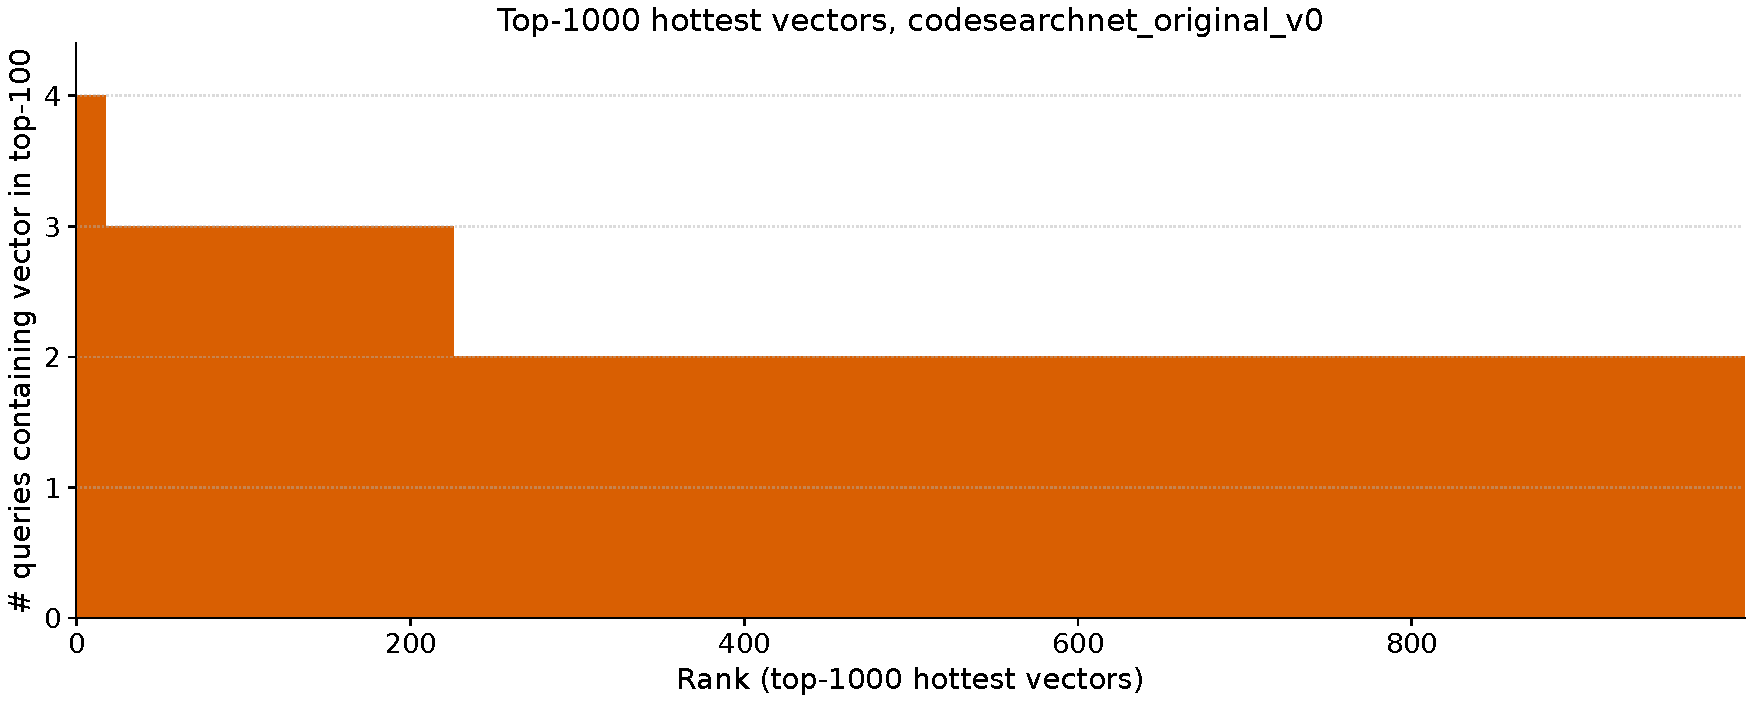
\includegraphics[width=\linewidth]{Figures/vector_hotness_top1000_codesearchnet_original_v0.pdf}
    \caption{Vector hotness for original, measured as the number of
    benchmark queries that include a given vector in their top-100
    ground-truth set.}
    \label{fig:hotness}
\end{figure}
\begin{figure}[t]
    \centering
    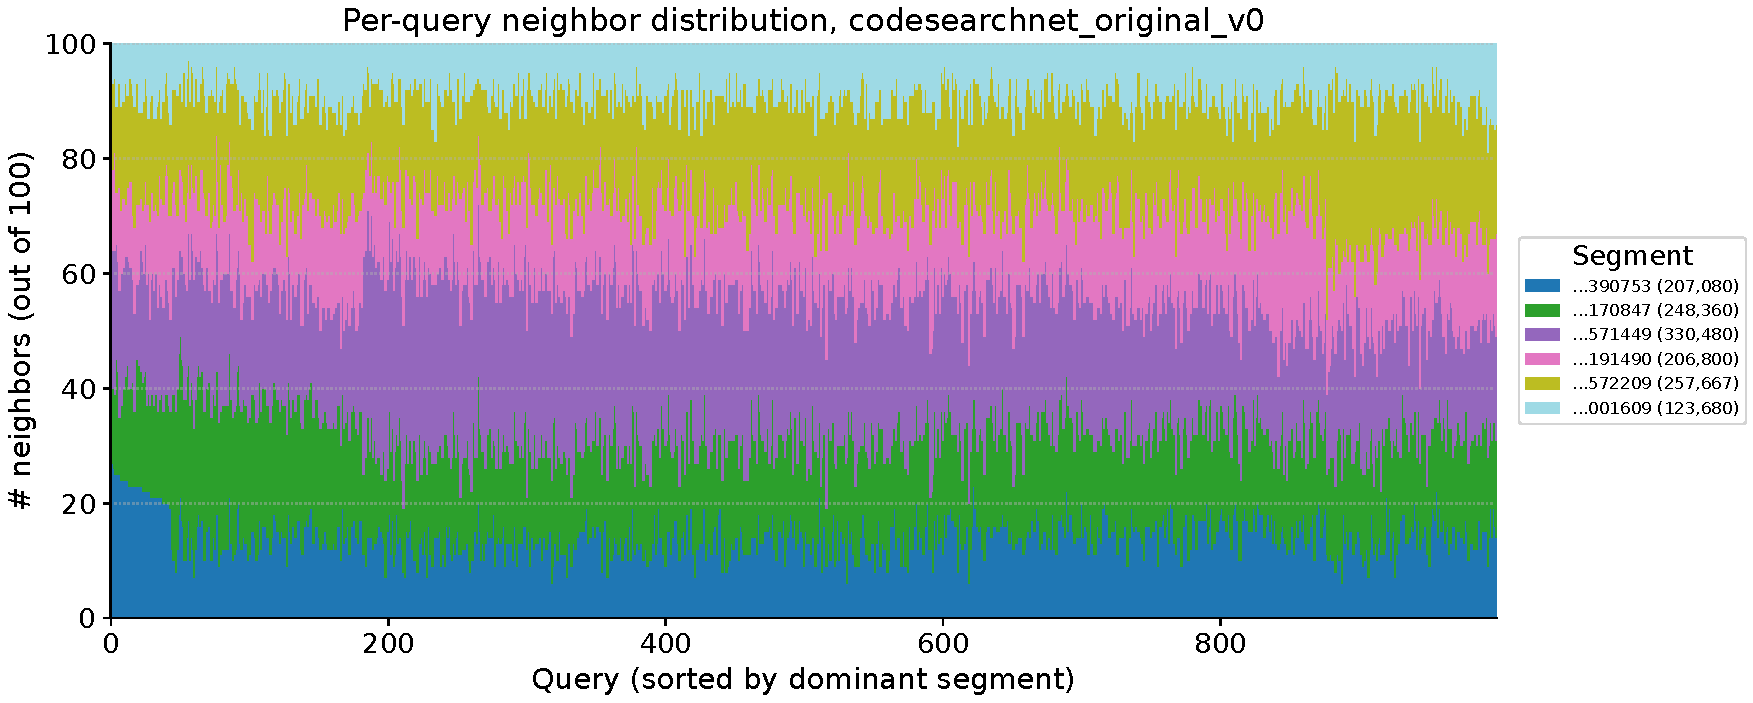
\includegraphics[width=\linewidth]{Figures/query_neighbor_segments_stacked_codesearchnet_original_v0.pdf}
    \caption{Per-query distribution of top-100 ground-truth neighbors
    across segments of the original collection. Each bar is a query,
    sorted by its dominant segment, each color is one segment. Most
    queries pull neighbors from several segments rather than a single
    hot one.}
    \label{fig:query-segments}
\end{figure}


\begin{figure}[t]
    \centering
    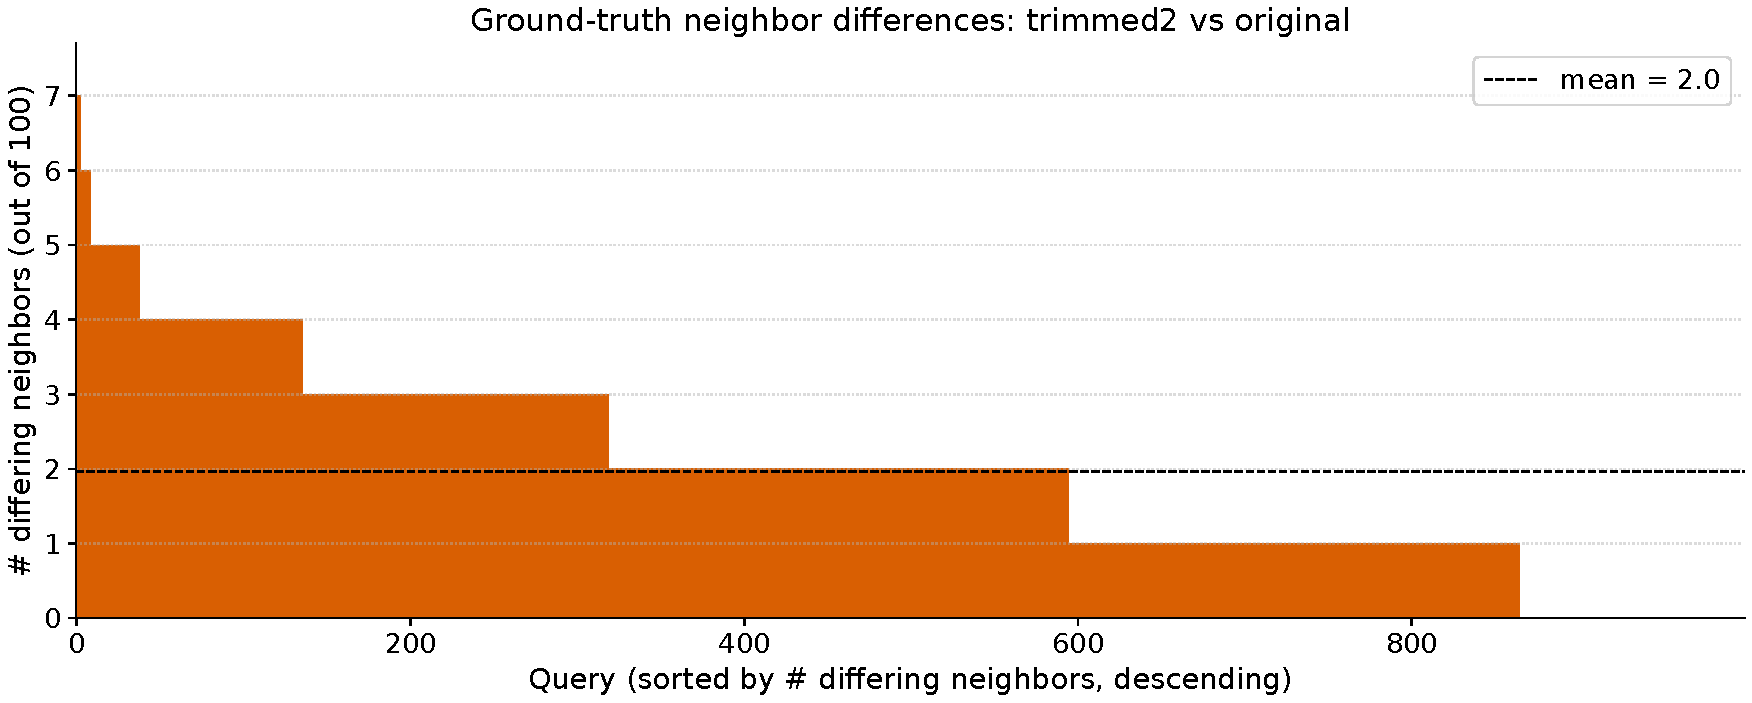
\includegraphics[width=\linewidth]{Figures/query_diff_trimmed2_vs_original.pdf}
    \caption{Per-query count of differing top-100 ground-truth neighbors
    between trimmed2 and original, sorted descending.}
    \label{fig:query-diff}
\end{figure}

Before looking at how Milvus stores the two collections on disk, we
first establish two properties of the workload that motivate asking the
question in the first place.



\mypar{Most vectors are never queried, and the accessed ones are
broadly dispersed.} \autoref{fig:hotness} plots, for each of the top-1000
most frequently accessed vectors, how many of the 1{,}000 benchmark
queries include it in their top-100 ground-truth list. The maximum
per-vector hit count is only 4 and the curve is essentially flat,
meaning no single vector is significantly hotter than any other. At the
corpus level, roughly 92\% of all vectors never appear in any query's
top-100 list, which is expected given that the benchmark returns 100
neighbors per query across approximately one million corpus vectors, so
the reachable fraction is on the order of
$100 \times 1{,}000 / 10^6 \approx 10\%$ before accounting for overlap
across queries. \autoref{fig:query-segments} then characterizes where
the touched vectors reside: for each query it counts how many of the
100 ground-truth neighbors fall into each segment of the original
collection. Neighbors are distributed across many segments per query
rather than bunched into one or two, so the ground-truth top-100 set is
broadly dispersed across the storage layout.


\mypar{The two collections answer most queries with the same neighbors.}
\autoref{fig:query-diff} compares the top-100 ground truth neighbor
lists between trimmed2 and original after remapping trimmed2 IDs into
the original index space. For the vast majority of queries the two
lists are identical or differ by only a handful of neighbors, and only
a small tail of queries sees substantial churn.
% At the workload level
% the two collections really are near-duplicates, so system that can
% align their segments has a real opportunity to serve both from shared
% data.

\subsection{Storage layout for near-identical collections}

\begin{figure*}[t]
    \centering
    \begin{subfigure}[t]{0.49\linewidth}
        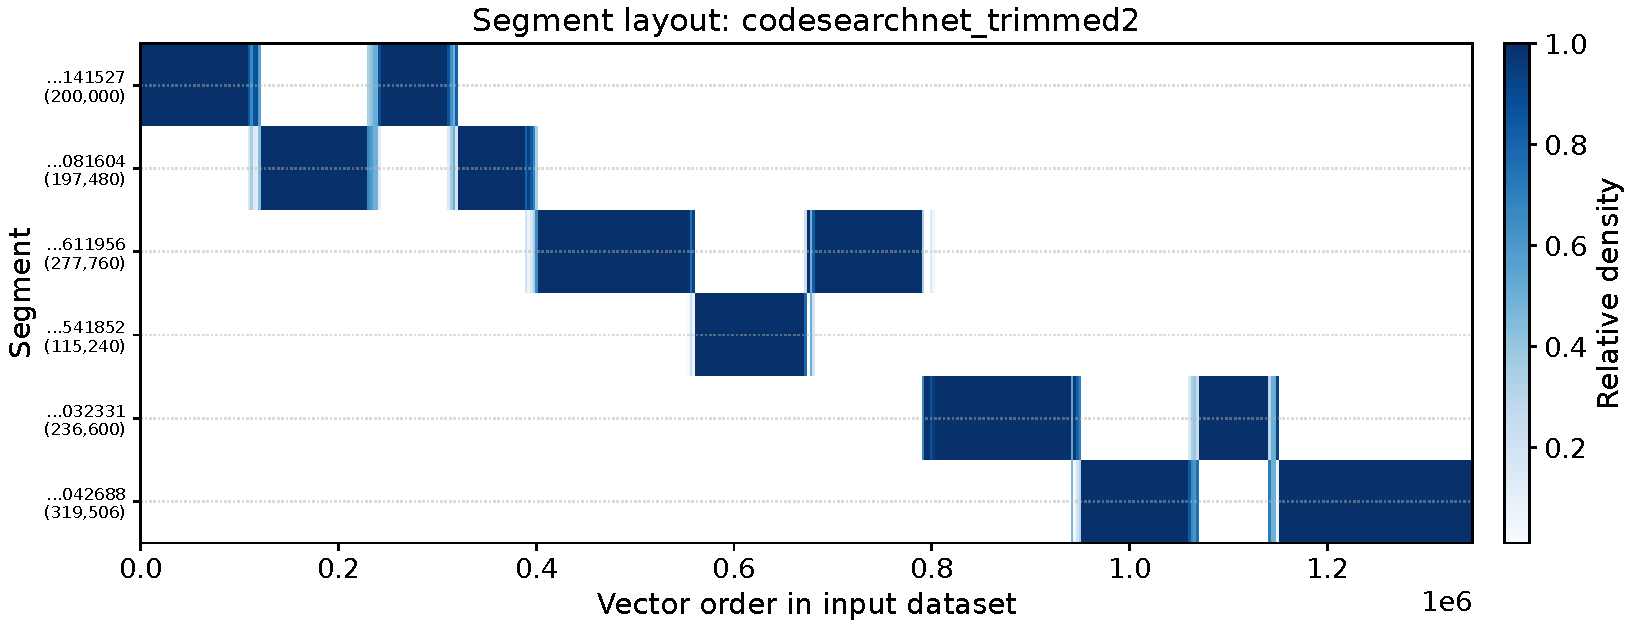
\includegraphics[width=\linewidth]{Figures/segment_layout_codesearchnet_trimmed2_bothOn.pdf}
        \caption{bothOn (stock Milvus).}
    \end{subfigure}\hfill
    \begin{subfigure}[t]{0.49\linewidth}
        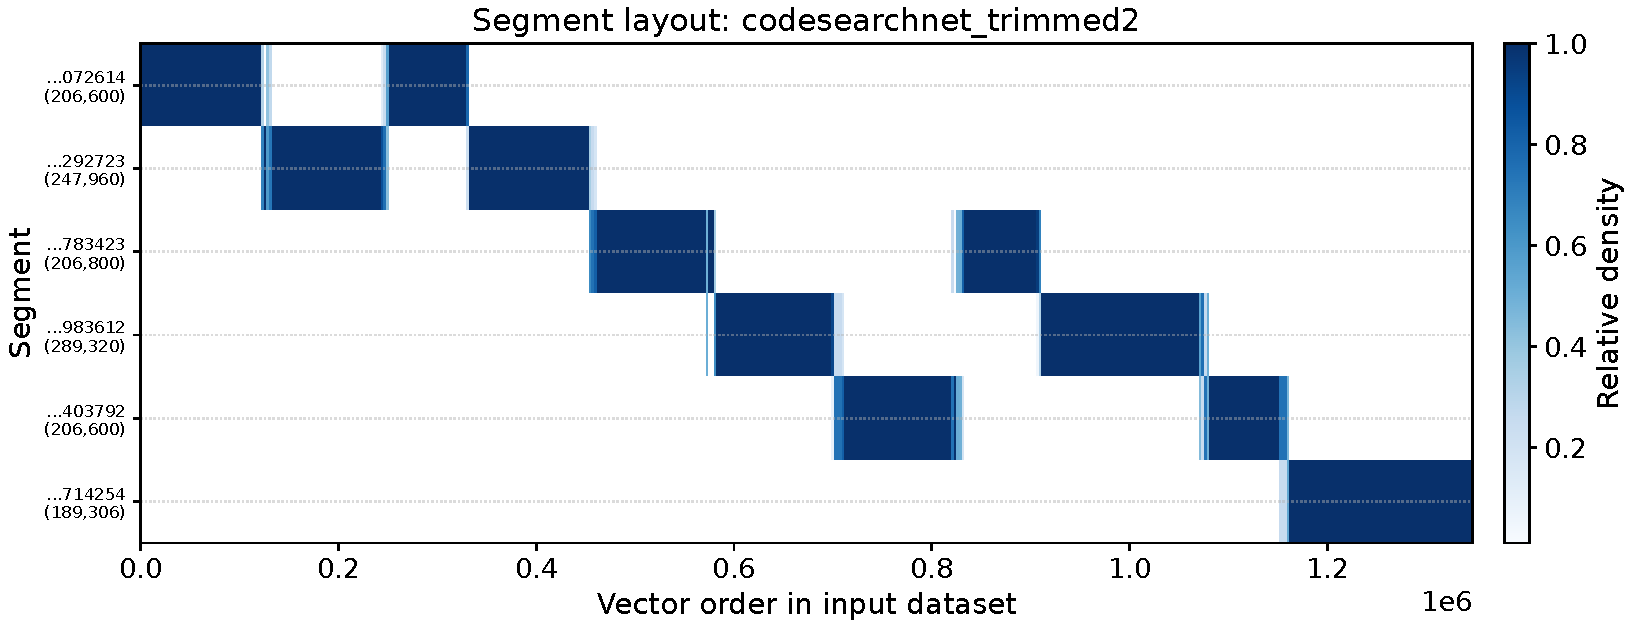
\includegraphics[width=\linewidth]{Figures/segment_layout_codesearchnet_trimmed2_nojitter.pdf}
        \caption{nojitter.}
    \end{subfigure}
    \caption{Segment layout of the trimmed2 collection. The X axis is the
    vector index in the input dataset and each row is one segment; darker
    cells indicate more vectors at that index landing in that segment.}
    \label{fig:segment-layout}
\end{figure*}

\begin{figure*}[t]
    \centering
    \begin{subfigure}[t]{0.33\linewidth}
        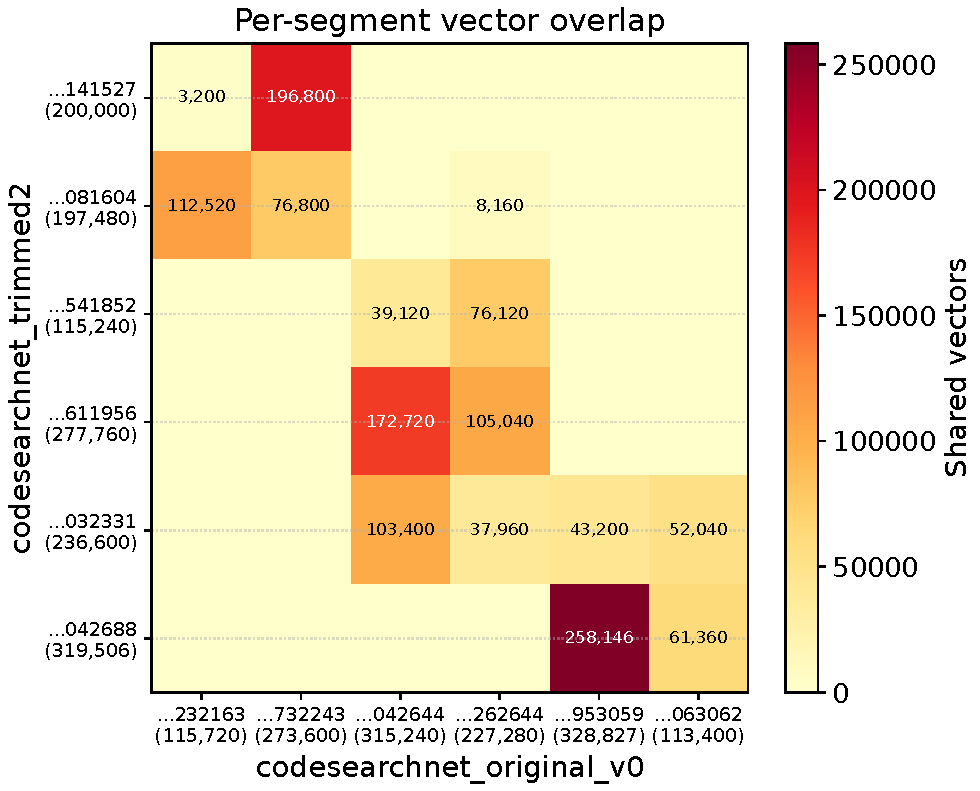
\includegraphics[width=\linewidth]{Figures/segment_overlap_codesearchnet_trimmed2_vs_codesearchnet_original_v0_bothOn.pdf}
        \caption{bothOn.}
    \end{subfigure}\hfill
    \begin{subfigure}[t]{0.33\linewidth}
        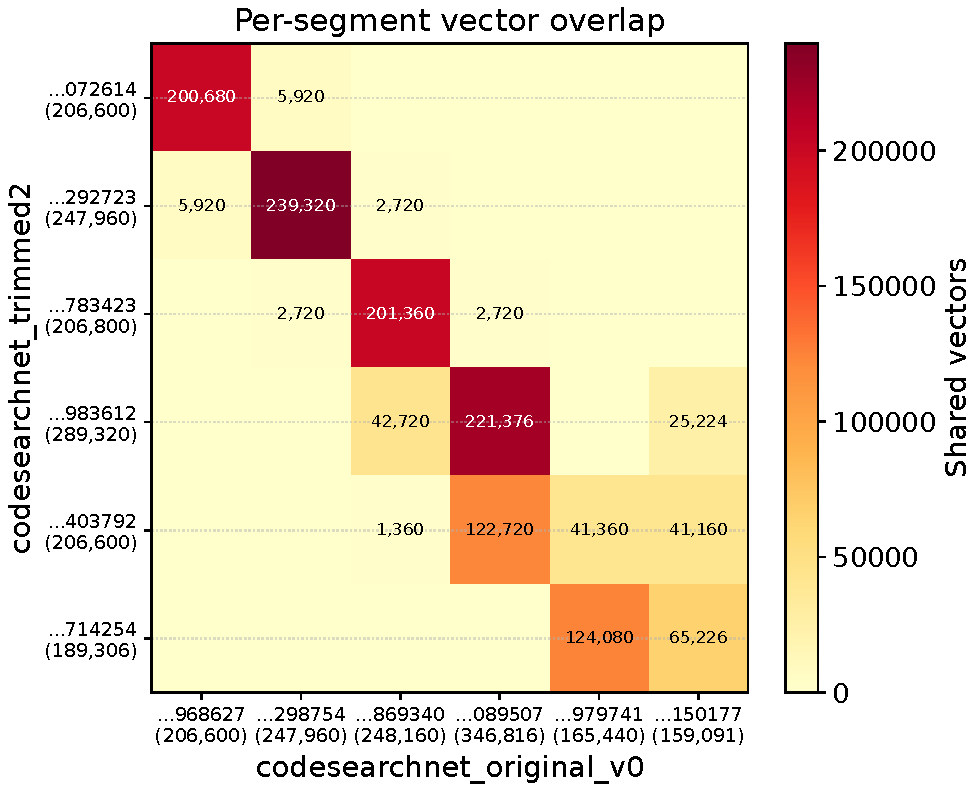
\includegraphics[width=\linewidth]{Figures/segment_overlap_codesearchnet_trimmed2_vs_codesearchnet_original_v0_nojitter.pdf}
        \caption{nojitter.}
    \end{subfigure}\hfill
    \begin{subfigure}[t]{0.31\linewidth}
        \raisebox{1.5mm}{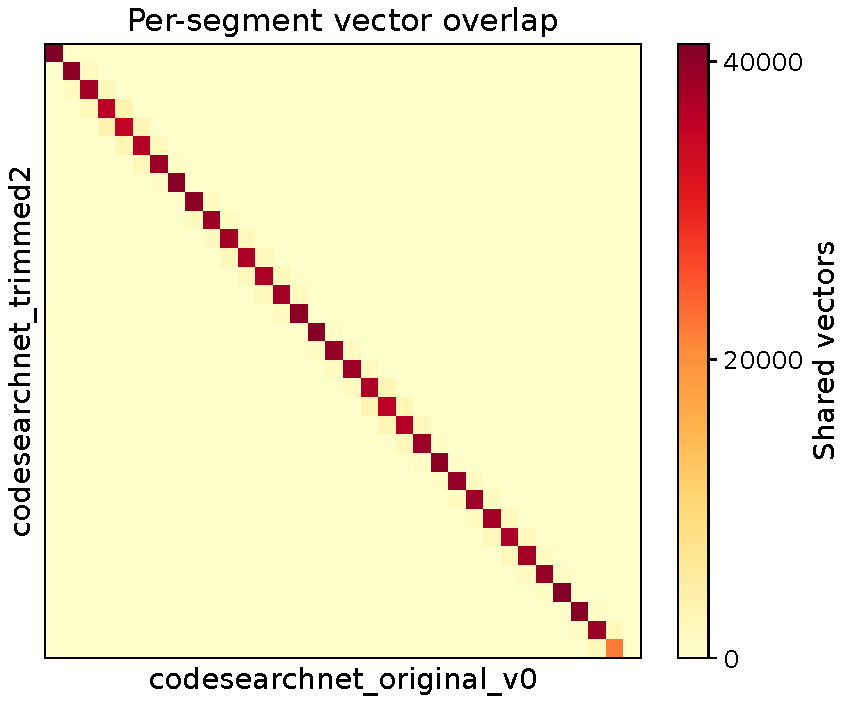
\includegraphics[width=\linewidth]{Figures/segment_overlap_codesearchnet_trimmed2_vs_codesearchnet_original_v0_noJitterCompaction.pdf}}
        \caption{noJitterCompaction.}
    \end{subfigure}
    \caption{Per-segment vector overlap between the trimmed2 and original
    collections. Rows are trimmed2 segments, columns are original segments,
    color encodes the number of shared primary keys.}
    \label{fig:segment-overlap}
\end{figure*}

Given a workload where the two collections are near-duplicates at the
query level, we now ask how Milvus~\cite{wang2021milvus} actually lays
them out on disk. Milvus organizes a collection as a sequence of
segments that are flushed from a write-ahead buffer, and a background
compactor may later merge small segments~\cite{guo2022manu}.

\mypar{Compaction, not jitter, is the main source of non-contiguous
segments.} \autoref{fig:segment-layout} shows, for the trimmed2
collection, which vector ranges of the input dataset end up in each
segment. Neither configuration produces a clean staircase. Under stock
Milvus (bothOn), each segment covers several disjoint bands of the
input vector space, and the bands themselves are smeared because the
jittered flush size makes different flushes seal at different vector
counts. Disabling jitter (nojitter) makes each band somewhat cleaner, but a
single segment still draws from two or more such strips, so even
without jitter the vector ranges held by a segment
are not contiguous. The reason is that compaction is still running:
the background compactor merges earlier-flushed segments into new
ones, and because those earlier segments were themselves flushed at
different points in the insert stream, the merged segment ends up
holding vectors from multiple non-adjacent input ranges. Jitter therefore
controls only the fuzziness of each strip, whereas the gap between the
two strips that share a segment is controlled by compaction.

\mypar{Cross-collection overlap is only meaningful under
noJitterCompaction.} \autoref{fig:segment-overlap} shows the
per-segment overlap matrix between the trimmed2 and original
collections for each of the three configurations. Each cell records the
number of vectors that a segment in trimmed2 (row) shares with a
segment in original (column). With stock Milvus, the matrix is dense
and scattered: shared vectors are smeared across many segment pairs, so
picking any single segment of the second collection only recovers a
small fraction of the vectors that a segment of the first holds. The
scatter is amplified by how jitter interacts with compaction: Milvus
selects which small segments to merge based on their sizes, and because
jitter produces differently sized segments across the two collections,
the compactor makes different merging choices for each, further
diverging their segment boundaries even when the underlying data is
nearly identical. Disabling jitter helps because it makes the first several compaction
choices identical across the two collections, which narrows each band
in the overlap matrix. However, as the number of remaining small
segments shrinks and their sizes approach the merge threshold, the
compactor's size-based selection hits a boundary where a small
difference tips the choice of which segments to merge, so the matrix
is still noisy in the nojitter configuration. With noJitterCompaction the overlap
collapses to a near-diagonal structure, where each trimmed2 segment has
one matching original segment and the shared region accounts for the
bulk of its vectors. The small offset along the diagonal is exactly the
2\% of vectors trimmed2 dropped from the head of the corpus. We also ran
the same comparison for two independent copies of the original
collection
% (\texttt{original\_v0} vs \texttt{original\_v1}) 
 and got
qualitatively identical behavior, which means the shuffling is inherent
to Milvus's ingest path and not specific to the trimmed workload.

\subsection{Storing in partitions within one collection}

\begin{figure}[t]
    \centering
    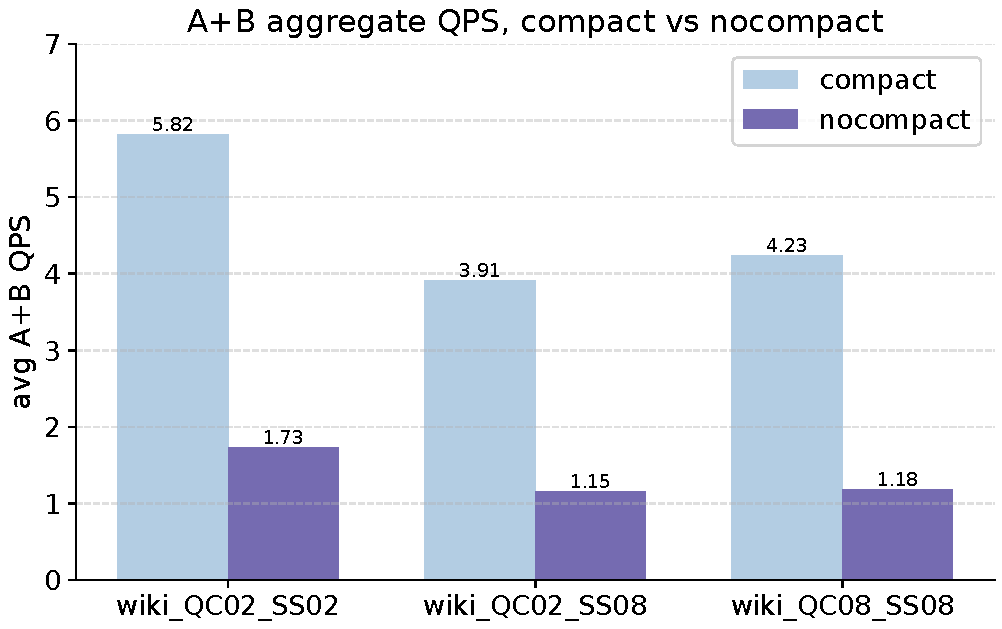
\includegraphics[width=\linewidth]{Figures/qps_compact_vs_nocompact.pdf}
    \caption{Aggregate $A$+$B$ concurrent QPS for the three Wikipedia
    workload variants, with compaction enabled and disabled.
    Compaction yields a roughly $3\times$ improvement across all
    variants.}
    \label{fig:qps-compact-vs-nocompact}
\end{figure}

\begin{figure}[t]
    \centering
    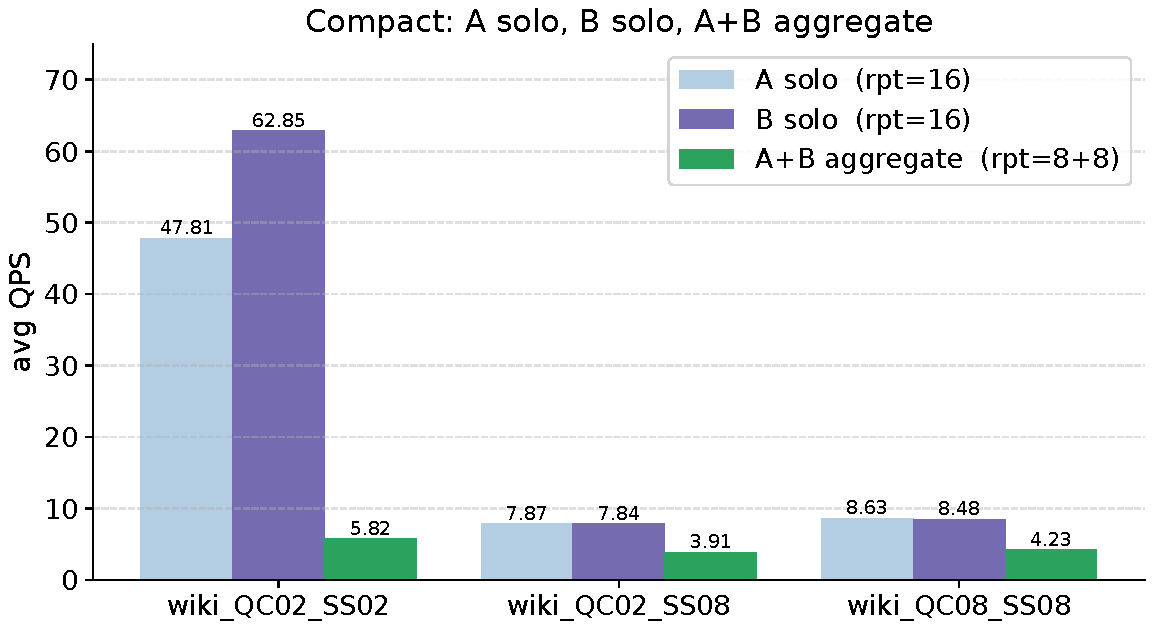
\includegraphics[width=\linewidth]{Figures/qps_compact_solo_vs_concurrent.pdf}
    \caption{Solo per-tenant QPS versus aggregate concurrent QPS on
    each compacted variant. On QC02\_SS02 the gap between solo and
    concurrent throughput exceeds an order of magnitude, while the
    QC*\_SS08 variants are already disk-bound in the solo case.}
    \label{fig:qps-solo-vs-concurrent}
\end{figure}

\begin{figure}[t]
    \centering
    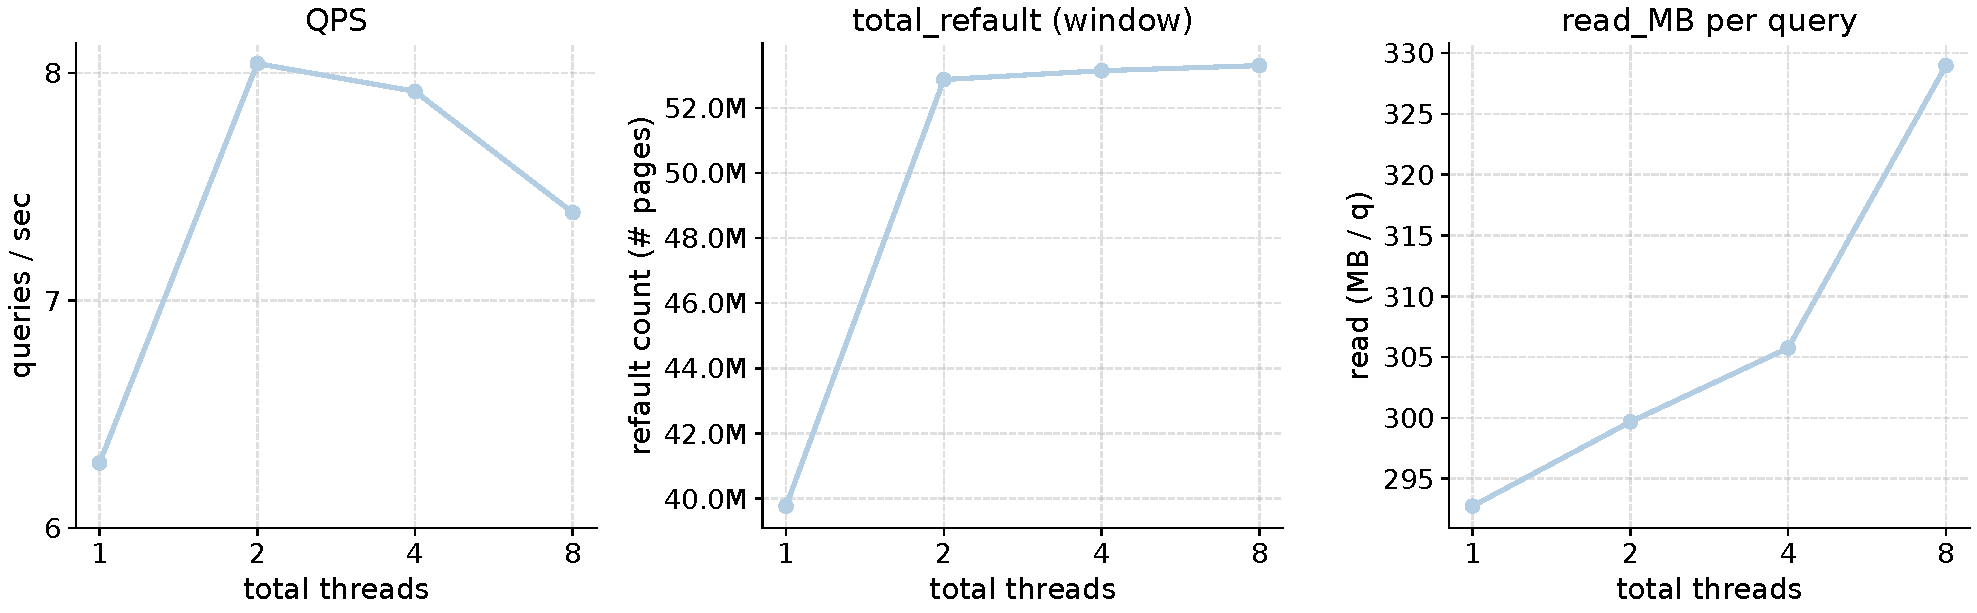
\includegraphics[width=\linewidth]{Figures/cache_miss_metrics_wiki_QC02_SS08.pdf}
    \caption{QPS, major page faults, and read volume per query as a
    function of total query threads on QC02\_SS08\_nocompact. Stable
    refault counts paired with rising per-query reads and falling QPS
    are the signature of page-cache thrashing.}
    \label{fig:cache-miss-metrics}
\end{figure}

The shared partition layout removes the storage redundancy of the
fully replicated layout by keeping a single collection in which the
shared corpus and each tenant's private vectors live in distinct
partitions. The open question for this layout is whether the
resulting resource sharing translates into competitive query
throughput once tenants query their respective tenant partitions
concurrently. We measure throughput along two axes: the effect of
compaction on aggregate concurrent throughput, and the per-tenant
throughput under solo and concurrent execution. We then drill into
a single configuration to identify the bottleneck that limits
concurrent performance.

\mypar{Compaction roughly triples aggregate throughput.} For each of
the three Wikipedia workload variants, we issue queries from both
tenants concurrently and report the aggregate QPS of $A$ and $B$
combined in \autoref{fig:qps-compact-vs-nocompact}. With compaction
enabled, the aggregate throughput is 5.82, 3.91, and 4.23 QPS for
QC02\_SS02, QC02\_SS08, and QC08\_SS08 respectively. Disabling
compaction drops the same numbers to 1.73, 1.15, and 1.18 QPS, a
factor of roughly $3\times$ across all three variants. The mechanism is straightforward: compaction merges many
small sealed segments into a smaller number of larger ones, so each
query fans out to fewer segments at search time and the working set
spans fewer page-cache pages. The compaction-disabled collections,
which carry roughly three times as many segments at the same total
vector count, force every query to scan more index files and pull more
pages off disk per request.

\mypar{Concurrent execution collapses solo throughput by an order of
magnitude.} \autoref{fig:qps-solo-vs-concurrent} contrasts each
tenant's solo throughput with the aggregate concurrent throughput on
the compacted collections. On QC02\_SS02 tenant $A$ alone reaches
47.81~QPS and tenant $B$ alone reaches 62.85~QPS, but running both
tenants concurrently yields a combined throughput of only 5.82~QPS,
roughly an order of magnitude below either solo case. The reason is
that QC02\_SS02 places 14.2M vectors in each tenant partition, and the
per-tenant working set comfortably fits in the 96\,GB RAM cap when
only one tenant is active. Once the second tenant joins and brings
its own 14.2M vector partition into active rotation, the combined
working set overflows the RAM cap and the page cache begins evicting
pages that the first tenant will read again on its next query. On
the two QC*\_SS08 variants, where 80\% of cold vectors live in the
shared partition and the tenant partitions are only 3.7 to 3.9M
vectors, solo throughput is already low at roughly 8~QPS because each
query must traverse the much larger shared partition, and even a
small tenant partition is enough to halve concurrent throughput once
both tenants are active. Whether a query could in principle be
answered entirely within the shared partition or entirely within
its tenant partition does not change the throughput observed on the
QC*\_SS08 variants, because the current search path is content
agnostic: every query fans out to all segments in the shared
partition and in its tenant partition, scans each one, and merges
the results, regardless of where the actual top-$k$ neighbors
reside. As a result, QC02\_SS08 and QC08\_SS08, which differ only
in how concentrated the top-$k$ neighbors are inside the shared
partition, exhibit essentially the same throughput under
concurrent execution.

\mypar{Scalability is bounded by page-cache thrashing, not CPU.} To
pin down the bottleneck, we sweep the number of query threads issued
against tenant $A$ on the QC02\_SS08\_nocompact collection, whose
relevant partition set comprises 240 segments, and track QPS, major
page fault count, and read volume per query as shown in
\autoref{fig:cache-miss-metrics}. QPS rises from 5.5~q/s at one
thread to 8.1~q/s at two threads, then \emph{falls} to 7.3~q/s at
eight threads, so adding concurrent requests actively reduces
throughput rather than scaling the system. The major page
fault count plateaus at roughly 53M pages across two, four, and
eight threads, indicating that the disk page-read rate is saturated
and is the binding ceiling rather than the CPU. The total read
volume per query, in contrast, keeps climbing from 293\,MB at one
thread to 329\,MB at eight threads, because each query increasingly
re-reads pages that a different concurrent query has just evicted
from the page cache. Stable refault counts, rising per-query read
volume, and falling QPS together form the classical signature of
page-cache thrashing, and they confirm that the shared partition
layout's performance ceiling under concurrency is dictated by how
the segment-level working set interacts with the page cache rather
than by the cost of index search itself.

\section{Conclusion and Next Steps}

The study leaves us with three observations that together frame the
design space for a multi-tenant vector store.

\mypar{Search is per segment in parallel.} Vectors are arranged
into sealed segments, and every query fans out to all of them,
scans each local index, and merges the partial results into a
global top-$k$. Per-query cost scales with both the number of
segments and the size of each segment's index, so any sharing
strategy must either reduce the number of segments a query
consults or amortize per-segment cost across tenants.

\mypar{Same data does not imply same segments.} Identical
logical data loaded into two collections produces different
segment cuts in stock Milvus, because flush jitter and background
compaction shuffle vectors across segment boundaries during
ingestion. Disabling both sources of non-determinism collapses
the per-segment overlap matrix to a diagonal, but the index and
data files within each segment still diverge across loads.
Vector-level overlap is therefore necessary but not sufficient
for sharing storage; a layout that makes segments byte-comparable
across collections by construction is required before sharing
can be exploited end to end.

\mypar{Sharing a collection has a real cost.} Co-locating
tenants in a single collection through a shared partition
removes the storage duplication of the fully replicated layout,
but query throughput under concurrent traffic collapses by an
order of magnitude relative to the solo case. The bottleneck is
not CPU but the page cache: the combined working set overflows
RAM and queries refault pages that concurrent queries have just
evicted, so the system enters a thrashing regime in which adding
threads reduces throughput. A workable shared layout must
therefore be paired with a memory allocation strategy that
bounds cross-tenant interference rather than relying on the
operating system page cache.

\mypar{Next steps.} These observations point to three follow-up
directions:
\begin{enumerate*}[label=(\arabic*)]
    \item \textbf{Make the search path content aware,} so that a
    query is routed only to the segments that hold its candidate
    top-$k$ neighbors rather than fanned out to every segment,
    and quantify how much per-segment HNSW~\cite{malkov2018hnsw}
    work could additionally be reused across tenants whose
    queries hit the same segments;
    \item \textbf{align segments by construction,} replacing
    implicit ingestion-time alignment with an explicit
    content-addressed segment layout, so that two collections
    with overlapping data share the same segment files rather
    than two independently flushed copies;
    \item \textbf{bound cross-tenant memory contention,}
    developing a memory allocation policy for shared-partition
    collections that reserves working-set budget per tenant or
    per partition, and extending the evaluation beyond two
    tenants.
\end{enumerate*}



\newpage
\bibliographystyle{plain}
\bibliography{reference}


\end{document}